\chapter{شبیه سازی و نتایج}\label{ch:resault}
در فصل‌های گذشته در خصوص ابزار هایی که در این پروژه استفاده شده‌اند، صحبت شد و توضیح مفصلی بر چیستی آن ابزار ها و ضرورت استفاده از آن‌ها داده شد. اما سوالات بی‌جوابی نیز ماند که در این فصل به آن ها خواهیم پرداخت.

یکی از آن سوالات نحوه راه‌اندازی کد پروژه می‌باشد و سوال دیگر نتیجه حاصل از شبیه سازی نهایی چگونه است می‌باشد.
\section{راه‌اندازی}\label{ch:resault|sec:launch}
این کد در گیت هاب در دو 
\w{repo}
قرار دارد.
جدول 
\ref{tab:github-myrepos}
اطلاعات این \w{repo}ها
\RTLfootnote{غیر از این دو \w{repo}، \w{repo} دیگری به آدرس زیر وجود دارد که تاریخچه و روند رسیدن به این نتیجه نهایی را نشان می‌دهد.
\url{https://github.com/MohammadRaziei/Prescan_test}
}
 را نشان می‌دهد.
\RTLfootnote{
آدرس این \ws{repo} به این شکل بدست می‌آید : \LRE{\texttt{https://github.com/mohammadraziei/<REPOSITORY-NAME>}} 
}
 
\begin{table}\tableset{
\begin{tabular}{|c|p{0.46\linewidth}|c|}
	\hline\rowcolor{lightgray}
	نام \w{repo} & توضیحات & نیاز به \w{matlabengine} \\\hline\hline
\texttt{gym-Prescan} &  
پروژه کامل در این \ws{repo} قرار دارد. در آن بر بخش الگوریتم از کتابخانه هایی استفاده شده است که بر روی سیستم عامل لینوکس قابل اجرا هستند بنابراین در صورتی که از لایه الگوریتمی که این پروژه از آن استفاده می‌کند استفاده نشود، در هر سیستم عاملی می‌توان از آن استفاده کرد.
  & \cmark \xmark \\\hline
\texttt{gym-Prescan-minimal} &  در این جا بخش فایل های \w{prescan} به همراه فایل هایی که به \w{matlabengine} نیاز  دارد حذف شده است.  & \xmark \\\hline
\end{tabular}}
\caption{اطلاعات \ws{repo}های پروژه در گیت‌هاب}
\label{tab:github-myrepos}
\end{table}

 ابتدا پیش‌نیاز های لازم را که در بخش
\ref{ch:req}
توضیح داده شدند، را نصب کنید. پیشنهاد می‌شود که تمامی نسخه‌های لازم توضیح داده شده در بخش \ref{ch:req} را در سیستم‌عامل لینوکس استفاده کنید. 

اگر به توصیه استفاده از لینوکس عمل نکرده باشید، می‌توانید با استفاده شبکه که کد در اختیارتان قرار می‌دهد کد را روی دو کامپیوتر اجرا کنید به طوری که در یک کامپیوتر ویندوز و نرم افزار های گفته شده نصب باشد و روی دیگری لینوکس و پایتون و پیشنیاز های پایتون که در بخش 
\ref{ch:req|sec:python-req}
بررسی شدند نصب باشد. 
\begin{note}
بهتراست این دو کامپیوتر در یک شبکه داخلی به یک دیگر متصل شده باشند.
\end{note}

حال وارد کامپیوتری شوید که ویندوز بر روی آن نصب است. این کامپیوتر قرار است نقش 
\w{env}
را برای ما ایجاد کند. 
\begin{note}
	کد های پایتون صرفا بر روی کامپیوتری که لینوکس دارد اجرا کنید.
\end{note}
 که دستور زیر را در \w{terminal} خود وارد کنید.

\begin{latin}
\begin{lstlisting}[language=bash]
git clone https://github.com/MohammadRaziei/gym-Prescan.git
pip install -e gym-Prescan
\end{lstlisting}
\end{latin}

خط دوم این کد، اختیاری می‌باشد و صرفا کار را ساده می‌کند. همچنین می‌توان آن را به صورت زیر نیز نوشت:

\begin{latin}
\begin{lstlisting}[language=bash]
pip install git+https://github.com/MohammadRaziei/gym-Prescan
\end{lstlisting}
\end{latin}

سپس وارد مسیر زیر شوید.
\begin{center}
\begin{latin}
gym-Prescan/gym\_prescan/envs/PreScan
\end{latin}
\end{center}

سپس با استفاده از آیکون 
\raisebox{-0.25\height}{
\includegraphics[width=1.2em]{Figures/PreScan-logo.png}}
\RTLfootnote{
این آیکون پس از نصب نرم‌افزار \w{prescan} بر روی دستکتاپ تشکیل می‌شود.
}
کلیک کنید. در این صورت برروی نوار \lr{Toolbar} این آیکون نیز ظاهر می‌شود. با فشردن آن،
 پنجره شکل 
\ref{fig:prescan-panel}
باز می‌شود. برروی \lr{Matlab} کلیک کنید تا محیط متلب باز شود. اچرای فایل \texttt{startup.m} برای هنگامی که از کد پایتون بر روی همان سیستم استفاده نمی‌کنید، اختیاری است. 

فایل سیمولینک را باز کنید و به صورت دستی \lr{IP} بلوک فرستنده را به \lr{IP} مورد نظر تغییر دهید و یا با استفاده از کد زیر در کامندلاین متلب تغییرات لازم را انجام دهید.

\begin{latin}
\begin{lstlisting}[language=matlab]
ExperimentName = 'PreScan_Vissim_Python_0';
send_ip = 'localhost';
sys = load_system([ExperimentName '_cs']);
set_param([ExperimentName '_cs/Environment/Send Data'], 'remoteURL',['"' send_ip '"']);
save_system(sys);
\end{lstlisting}
\end{latin}

در این کد کافیست مقدار \texttt{send\_ip} را مطابق با \lr{IP} کامپیوتر دیگر تنظیم کنید. پس از تنظیمات فایل سیمولینک را اجرا کنید برای این کار می‌توانید آن را باز کرده و اجرا کنید و یا با استفاده از دستور زیر در کامندلاین متلب آن را انجام دهید.
\begin{latin}
\begin{lstlisting}[language=matlab]
ExperimentName = 'PreScan_Vissim_Python_0';
sys = load_system([ExperimentName '_cs']);
set_param(bdroot, 'SimulationCommand', 'start');
\end{lstlisting}
\end{latin}

حال در سیستم لینکوس خود میتوانید بسته زیر را دانلود کنید.

\begin{latin}
\begin{lstlisting}[language=bash]
git clone https://github.com/MohammadRaziei/gym-Prescan-minimal.git
cd gym-Prescan-minimal
\end{lstlisting}
\end{latin}

در این پوشه تعدادی از الگوریتم های معروفی که در حوزه \w{drl}(\gls{a:drl}) نوشته شده است، قرار دارد.
در بین این الگوریتم ها دو الگوریتم \gls{a:dqn} و \gls{a:a2c} نسبت به بقیه بهتر جواب داده اند. این الگوریتم ها در بخش 
\ref{ch:rl}
و در 
\cite{stable-baselines}
توضیح کامل داده شده‌اند.

برای اجرای الگوریتم \gls{a:dqn} باید ابتدا \lr{IP} کامپیوتر ویندوزی را در قسمت مشخص در متغیر \texttt{env\_dict} که در جدول \ref{tab:env-dict} به‌طور کامل بررسی شده است، بنویسید و سپس دستور \LRE{\texttt{python dqn.py}} را در \w{terminal} لینوکس وارد کنید. بدین صورت محیط شبیه‌سازی روی هر دو کامپیوتر شروع به کار می‌کند.



\section{نتایج شبیه‌سازی}

الگوریتم استفاده شده در این پروژه \gls{a:dqn} می‌باشد. این الگوریتم در بخش \ref{ch:alg}  بررسی شده است. همچنین در مرجع \cite{stable-baselines-doc} نحوه پیاده‌سازی آن توضیح داده شده است. مقدار $\gamma$ در این الگوریتم $0.8$ انتخاب شده است. یا توجه به \w{state} و  \w{reward} های تعریف شده در فصل \ref{ch:alg} پس از 400 بار تلاش به \w{optpol} می‌رسد.
اما برای بالا رفتن دقت ، 25000 بار \w{agent} مسیر را طی کرده است. دلیل آن بالا رفتن تعداد \w{episode}ها می‌باشد. با این کار مقدار $\epsilon$ کاهش یافته و احتمال جست و جوی \w{pol} جدید آن کاهش می‌یابد.

\begin{figure}
	\centering
	\subfigure[]{	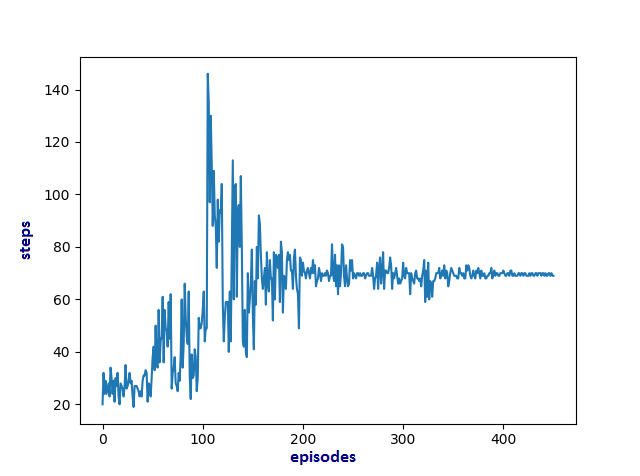
\includegraphics[width=0.4\linewidth]{Figures/code/step-episode-4}
		\label{subfig:step-episode}
	}
	\subfigure[]{
		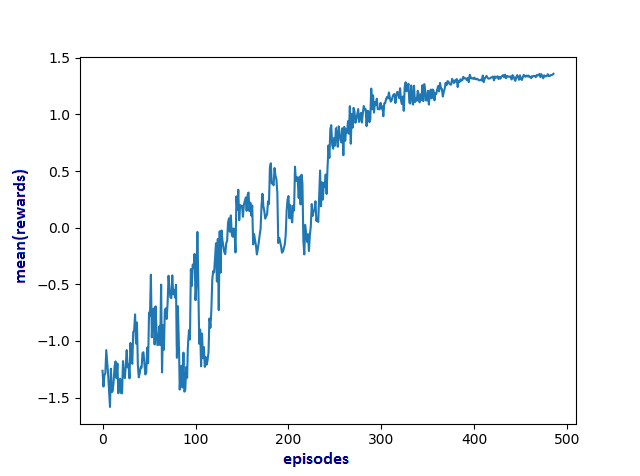
\includegraphics[width=0.4\linewidth]{Figures/code/reward-episode-4}
		\label{subfig:reward-episode}
	}
	\caption{نمودار توصیف رفتار \ws{agent} در هر \w{episode}}
	\label{fig:episode-chart}
\end{figure}

نمودار شکل \ref{subfig:reward-episode}، میانگین بدون وزن \w{reward} در پایان هر \w{episode} می‌باشد. در حوالی تا قبل از حدود 200 میانگین \w{reward} ها منفی است. زیرا تا قبل از آن، تصادف رخ می‌داد و در کل منفی بودش. شیب تقریبا صعودی آن در این مرحله بخاطر افزایش \w{step}ها می‌باشد که تاثیر منفی تصادف را کاهش داده است. در کل مشاهده می‌شود که روندی صعودی تا رسیدن به مقدار بیشینه \w{reward} دارد.

نمودار \ref{subfig:step-episode}، تعداد مراحل را در هر \w{episode} نشان می‌دهد. انتظار آن است که در ابتدا به دلیل تصادف کم باشد و در انتها روی مقدار مشخصی ثابت شود. حال ممکن است در این بین اتفاقاتی نیز افتاده باشد. یکی از اتفاقات جالب کاهش مقدار قله در شکل \ref{subfig:step-episode} می‌باشد. این مقدار با تنظیم مناسب پارامتر $\gamma$ کنترل شده است و مشاهده می‌شود که یک قله بیشتر ندارد و این یعنی آن \w{pol} را ادامه نداده است.

در نهایت، پس از یافتن \w{optpol}، تعداد \w{step}ها به 73 رسید. سرعت \w{agent} حول 21 در حال نوسان است و میانگین بدون وزن \w{reward}ها برابر $1.33821$ می‌باشد.

از آن‌جایی که نتایج این پروژه به صورت تصویر قابل بیان نیستند و نمی‌توان حتی چندین تصویر مختلف از وضعیت های مختلف آن گرفت و به عنوان نتیجه منتشر کرد، 
از نتایح این پروژه، فیلمی تهیه شده است که در آدرس زیر بارگذاری شده‌است.
\begin{center}
	\lr{\url{https://youtu.be/chgpBWU9XCA}}
\end{center}

همچنین فیلم دیگری نیز از روند اجرای این الگوریتم در سه بازه زمانی آماده شده است که آدرس آن نیز در زیر قرار دارد.

\begin{center}
	\lr{\url{https://youtu.be/JrDWDWqv1Hg}}
\end{center}



%\begin{figure}%[2]
%	\centering
%	\href{http://www.google.de}{\includegraphics{image}}
%	\caption{Non linked caption.}
%\end{figure}







\begin{figure}
	\centering
	\subfigure[]{
		\href{https://youtu.be/chgpBWU9XCA}{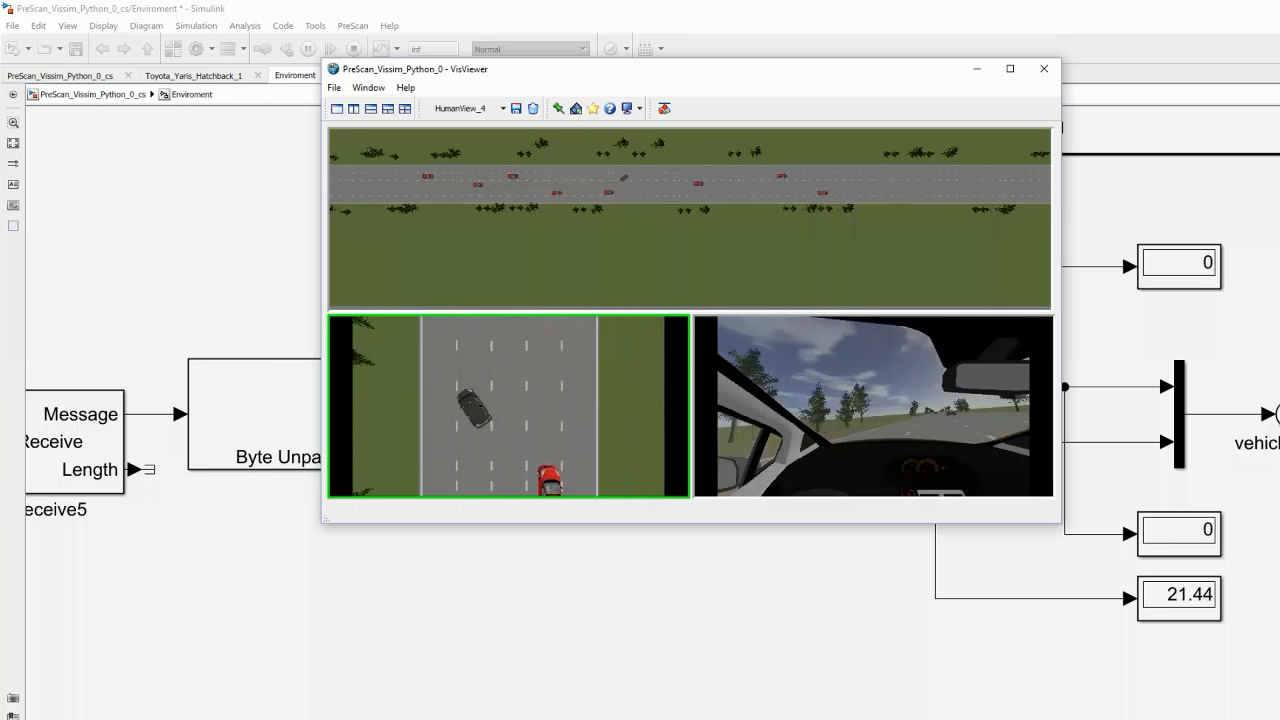
\includegraphics[width=0.7\linewidth]{Figures/OBS/resault}}
		\label{subfig:resault1}
	}
	\subfigure[]{
		\href{https://youtu.be/chgpBWU9XCA}{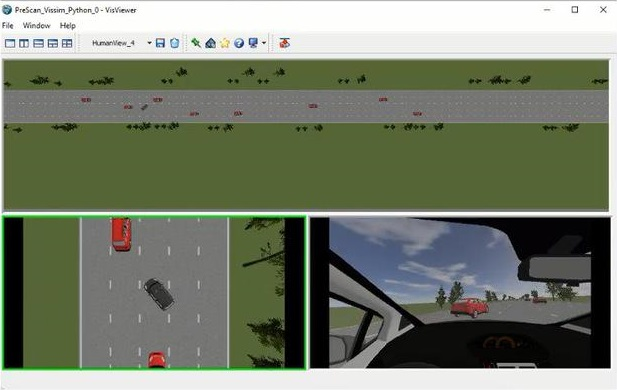
\includegraphics[width=0.7\linewidth]{Figures/OBS/resault2}}
		\label{subfig:resault2}
	}
	\caption[تصویر شبیه‌سازی نهایی]{
		شبیه سازی نهایی، شکلی مانند این دارد. از این رو فیلمی از این محیط درحال اجرا تهیه شده است که در آدرس
		\lr{\url{https://youtu.be/chgpBWU9XCA}}
		بارگذاری شده است.		
	}	
	\label{fig:resault}
	
\end{figure}
















